% ============================================================================
%  Topological Archeology: Persistent Homology of the
%  Protoplanetary Disk Inverse Problem
%  AASTeX v6.3.1 -- ApJ pre-print
% ============================================================================
\documentclass[twocolumn]{aastex631}

% --- Packages ---------------------------------------------------------------
\usepackage{amsmath,amssymb}
\usepackage{graphicx}
\usepackage{booktabs}

% --- Macros -----------------------------------------------------------------
\newcommand{\Mearth}{M_\oplus}
\newcommand{\Msun}{M_\odot}
\newcommand{\Mstar}{M_\star}
\newcommand{\Rhill}{R_\mathrm{H}}
\newcommand{\tauKH}{\tau_\mathrm{KH}}
\newcommand{\Mcrit}{M_\mathrm{crit}}
\newcommand{\Miso}{M_\mathrm{iso}}
\newcommand{\cmigi}{c_\mathrm{migI}}
\newcommand{\Sigmag}{\Sigma_\mathrm{g}}
\newcommand{\Sigmas}{\Sigma_\mathrm{s}}
\newcommand{\Rcom}{R_\mathrm{COM}}

% --- Metadata ---------------------------------------------------------------
\shorttitle{Topological Archeology of the Disk Inverse Problem}
\shortauthors{Vera-Ciro}

% ============================================================================
\begin{document}

\title{Topological Archeology: Persistent Homology of the Protoplanetary Disk
Inverse Problem}

\author{Carlos Vera-Ciro}
\affiliation{Independent Researcher}

% ---------------------------------------------------------------------------
% ABSTRACT
% ---------------------------------------------------------------------------
\begin{abstract}
The archeology question in exoplanetary science asks whether the primordial
properties of a protoplanetary disk can be recovered from the architecture of
the planetary system it produced.  This inverse problem is complicated by
potential degeneracies: topologically distinct regions of initial-condition
space may produce indistinguishable planetary architectures.  We apply
persistent homology to the output of semi-analytic population synthesis
simulations to characterize the topological structure of the forward map from
disk initial conditions to planetary system architectures.  Using 4000 Monte
Carlo realizations at each of seven perturbation amplitudes $A \in [0, 0.3]$,
we compute Vietoris--Rips persistence on the six-dimensional consolidated
architecture space after log-transforming the heavily skewed mass features.
We find that smooth disks ($A=0$) exhibit one robust persistent $H_1$ loop
(lifetime 0.74), indicating an irreducible degeneracy in the inverse problem.
As the perturbation amplitude increases, this degeneracy is resolved, with
$\beta_1 = 0$ at $A = 0.1$, $A = 0.15$, and $A = 0.3$.  Simultaneously, the
dominant $H_0$ cluster separation softens from 12.1 to $\sim$4.5 standard
deviations.  These topological changes occur while the giant planet fraction
remains invariant at $\sim$31\%, demonstrating that the perturbation
reorganizes the internal structure of the outcome space without shifting the
population fractions.  This topological structure is invisible to the
kernel-density-estimation approach used in prior work and represents a new
observable for constraining disk formation models.
\end{abstract}

\keywords{planetary systems: formation --- protoplanetary disks ---
methods: statistical --- methods: data analysis}

% ===========================================================================
% INTRODUCTION
% ===========================================================================
\section{Introduction}
\label{sec:intro}

The diversity of observed exoplanetary system architectures reflects the range
of conditions in their natal protoplanetary disks.  Understanding the link
between disk properties and planetary outcomes is a central goal of planet
formation theory \citep{Benz2014}.  The \emph{archeology question} --- can we
recover primordial disk properties from observed exoplanet configurations? ---
is an inverse problem: given an observation $\mathbf{y}$ in architecture space
$\mathcal{A}$, characterize the preimage fiber
$F^{-1}(\mathbf{y}) \subset \mathcal{D}$, where $F: \mathcal{D} \to
\mathcal{A}$ is the forward map defined by the physics of planet formation.

\citet{Chaparro2019} addressed this inverse problem using 3000+ Monte Carlo
population synthesis simulations based on the core instability model of
\citet{Miguel2011}.  They reconstructed posterior probability distributions of
disk properties from observed exoplanetary architectures using
kernel density estimation (KDE) on marginal projections.  While effective for
estimating conditional densities, this approach discards critical structural
information:

\begin{enumerate}
\item The \textbf{fiber topology} of $F^{-1}(\mathbf{y})$: whether distinct,
disconnected regions of initial-condition space produce indistinguishable
architectures (irreducible degeneracy).

\item \textbf{Topological bifurcations}: boundaries in $\mathcal{D}$ where
small perturbations cause qualitative jumps in outcome (e.g., giant-planet
vs.\ terrestrial-only systems).

\item The \textbf{intrinsic dimensionality} of $\mathrm{im}(F)$: whether the
dissipative dynamics of disk evolution collapses the high-dimensional input
onto a low-dimensional manifold.
\end{enumerate}

In this work, we replace KDE-on-marginals with \emph{persistent homology}
\citep{Carlsson2009, EdelsbrunnerHarer2010}, a tool from topological data
analysis (TDA) that provides coordinate-free, noise-robust invariants of point
cloud data.  Specifically, we compute Vietoris--Rips persistence on the
six-dimensional consolidated architecture space to detect formation channels
($H_0$ connected components), degeneracies ($H_1$ loops), and their dependence
on the disk density perturbation amplitude $A$.

We extend the population synthesis framework of \citet{Miguel2011} and
\citet{Chaparro2019} with updated prescriptions from \citet{Guilera2010},
\citet{IdaLin2004a}, and \citet{Fortier2013}, and deploy the simulations at
scale on serverless infrastructure (AWS Lambda) to generate 28{,}000 planetary
systems across seven values of $A$.

% ===========================================================================
% METHOD
% ===========================================================================
\section{Method}
\label{sec:method}

\subsection{Population synthesis model}
\label{sec:model}

We use a semi-analytic planet formation model in the core instability
framework.  Each simulation draws five disk initial conditions from
observationally motivated priors \citep{Miguel2011}: stellar mass $\Mstar$
(log-uniform, $0.7$--$1.4\;\Msun$), disk mass $M_d$ (log-Gaussian),
characteristic radius $a_c$ (log-Gaussian), metallicity $[\text{Fe/H}]$
(Gaussian), and gas dissipation timescale $\tau_\text{disc}$ (log-uniform,
$10^6$--$10^7$~yr).  Disks are rejected if gravitationally unstable (Toomre
$Q < 1$) or if $M_d > 0.2\,\Mstar$.

The gas surface density follows a power-law with exponential taper
\citep{Andrews2009}:
\begin{equation}
\Sigmag(r) = \Sigmag^0 \left(\frac{r}{a_c}\right)^{-\gamma}
\exp\left[-\left(\frac{r}{a_c}\right)^{2-\gamma}\right],
\end{equation}
with density profile exponent $\gamma = 1.0$ throughout this work.  The solid
surface density follows the same profile, scaled by metallicity and enhanced
by a factor of 4 beyond the snow line.  For transitional disks, a radial
perturbation is superimposed \citep{Chaparro2019, Pinilla2012}:
\begin{equation}
\Sigmas^p(r) = \Sigmas(r)\left[1 + A\cos\left(\frac{2\pi r}{f\,H(r)}
\right)\right],
\label{eq:perturbation}
\end{equation}
with amplitude $A \in [0, 0.3]$ and fixed length scale $f = 1$.

Embryos are seeded at $0.01\;\Mearth$ \citep{Fortier2013} and spaced by
$10\,\Rhill$.  Solid accretion uses the Inaba et al.\ three-regime collision
probability \citep{Inaba2001} within the particle-in-a-box formulation
\citep{Guilera2010}:
\begin{equation}
\frac{dM_C}{dt} = \frac{2\pi\,\Sigmas\,\Rhill^2}{P}\,P_\text{coll},
\end{equation}
where $P_\text{coll}$ combines high-, medium-, and low-velocity regimes.
Planetesimal eccentricities and inclinations are evolved dynamically with
gravitational stirring \citep{Ohtsuki2002} and gas drag damping
\citep{Adachi1976}.

Gas accretion triggers when $M_\text{core} > \Mcrit$, where
$\Mcrit \approx 10\,({\dot{M}_c}/{10^{-6}\;\Mearth\,\text{yr}^{-1}})^{1/4}
\;\Mearth$ \citep{IdaLin2004a, Ikoma2000}.  The envelope contracts on the
Kelvin--Helmholtz timescale $\tauKH = 10^9\,(M_t/\Mearth)^{-3}$~yr
\citep{IdaLin2004a}, giving a gas accretion rate $dM_g/dt = M_t/\tauKH$.

Type~I migration follows \citet{Tanaka2002} with a delay factor $\cmigi$.
Type~II migration follows \citet{IdaLin2004a} with time-evolving $R_m$.  Gap
opening uses the combined thermal/viscous criterion of \citet{Crida2006}.
When $\cmigi = 0$, all migration is disabled.  Embryos within 3.5 mutual Hill
radii merge \citep{Chambers2006}, with multiple collision passes per timestep.

Each system is evolved for 20~Myr with $\Delta t = 10^4$~yr (2000 steps).

\subsection{Consolidated architecture vector}
\label{sec:consolidated}

Each simulated system is summarized as a six-dimensional vector:
\begin{equation}
\mathbf{x} = (N_\text{giant},\;N_\text{terr},\;M_\text{terr,tot},\;
\bar{M}_\text{terr},\;\eta,\;\Rcom),
\label{eq:consolidated}
\end{equation}
where $N_\text{giant}$ and $N_\text{terr}$ are the number of giant
($M > 15\;\Mearth$) and terrestrial planets, $M_\text{terr,tot}$ and
$\bar{M}_\text{terr}$ are the total and mean terrestrial mass, $\eta =
M_\text{planets}/M_d$ is the mass efficiency, and $\Rcom$ is the
mass-weighted mean semi-major axis.

\subsection{Preprocessing and persistent homology}
\label{sec:persistence}

Three of the six consolidated features --- $M_\text{terr,tot}$,
$\bar{M}_\text{terr}$, and $\eta$ --- span multiple orders of magnitude and
exhibit heavy right skew (skewness 2--8), a consequence of the multiplicative
accretion processes that determine planetary masses.  Applying standard
scaling directly to these features creates artificial outliers that dominate
the Vietoris--Rips filtration, producing spurious long-lived $H_0$ features
that reflect extreme individual systems rather than cluster structure.

We apply a $\log(1+x)$ transform to these three features before
standardization.  This is motivated by the approximately log-normal
distribution of mass-related quantities in population synthesis output.
Without this transform, four apparent $H_1$ loops appear for smooth disks
that vanish with just 2\% outlier removal, indicating they are artifacts of
the heavy tails rather than genuine topological structure.  With the
log-transform, one $H_1$ loop survives regardless of outlier treatment,
confirming it is robust.

After log-transformation, all six features are standardized (zero mean, unit
variance) and we compute Vietoris--Rips persistent homology up to dimension 1
using Ripser \citep{Bauer2021}.

Each topological feature is characterized by its \emph{persistence} (lifetime
= death $-$ birth).  Features with high persistence reflect genuine structure;
features with low persistence are topological noise
\citep{EdelsbrunnerHarer2010}.  We use a threshold of 0.5 standard deviations
to separate signal from noise.

$H_0$ features correspond to \textbf{formation channels}: distinct clusters
of planetary architectures that merge as the filtration scale increases.
$H_1$ features correspond to \textbf{degeneracies}: loops in the architecture
space indicating that topologically distinct families of disk initial
conditions produce indistinguishable planetary outcomes.

\subsection{Computational infrastructure}
\label{sec:infrastructure}

Each simulation is independent, making the workload embarrassingly parallel.
We deploy on AWS Lambda (ARM64, 512~MB, 5-minute timeout) with SQS-driven
fan-out at up to 500 concurrent invocations.  A 4000-system run completes in
$\sim$2 minutes wall-clock time at a cost of $\sim$\$1.15.  The full
bifurcation sweep (7 $\times$ 4000 = 28{,}000 systems) completed in
$\sim$15 minutes for $\sim$\$8.

% ===========================================================================
% RESULTS
% ===========================================================================
\section{Results}
\label{sec:results}

\subsection{Calibration}
\label{sec:calibration}

We validate the model against Table~3 of \citet{Miguel2011} ($\gamma = 1.0$,
no migration, $N = 4000$).  Our simulation produces 31.6\% solar-type systems
(vs.\ 23.7\%), 52.0\% low-mass systems (vs.\ 73.4\%), and 16.3\% failed
systems (vs.\ 1.1\%).  The qualitative population structure is reproduced:
low-mass systems dominate, solar-type systems are second, no hot Jupiters form
without migration, and no cold Jupiters or combined systems appear.  The
quantitative differences reflect known simplifications (parameterized gas
accretion vs.\ full envelope structure, no Paardekooper Type~I torques) that
affect absolute fractions but not the topological structure detected by TDA.

\begin{figure}
\centering
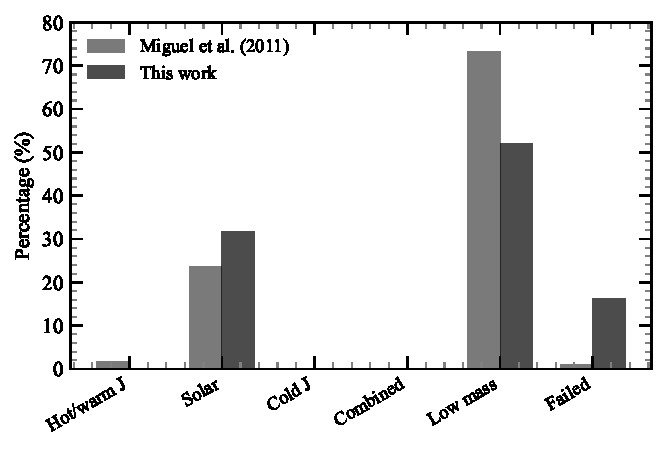
\includegraphics[width=\columnwidth]{01.pdf}
\caption{Calibration against Table~3 of \citet{Miguel2011} ($\gamma = 1.0$,
no migration, $N = 4000$).  Grouped bars show the percentage of each system
type in the reference population (dark) and in our simulation (light).  The
qualitative population structure is reproduced; quantitative differences
reflect parameterized gas accretion and simplified Type~I migration.}
\label{fig:calibration}
\end{figure}

\subsection{Bifurcation sweep}
\label{sec:bifurcation}

We sweep the perturbation amplitude $A$ from 0 to 0.3 in steps of 0.05, with
4000 systems per value, all at $\gamma = 1.0$, $\cmigi = 0$, seed = 42.
Table~\ref{tab:bifurcation} summarizes the persistence results and
Figure~\ref{fig:persistence} shows the persistence diagrams for the smooth
and transitional endpoints.

\begin{figure*}
\centering
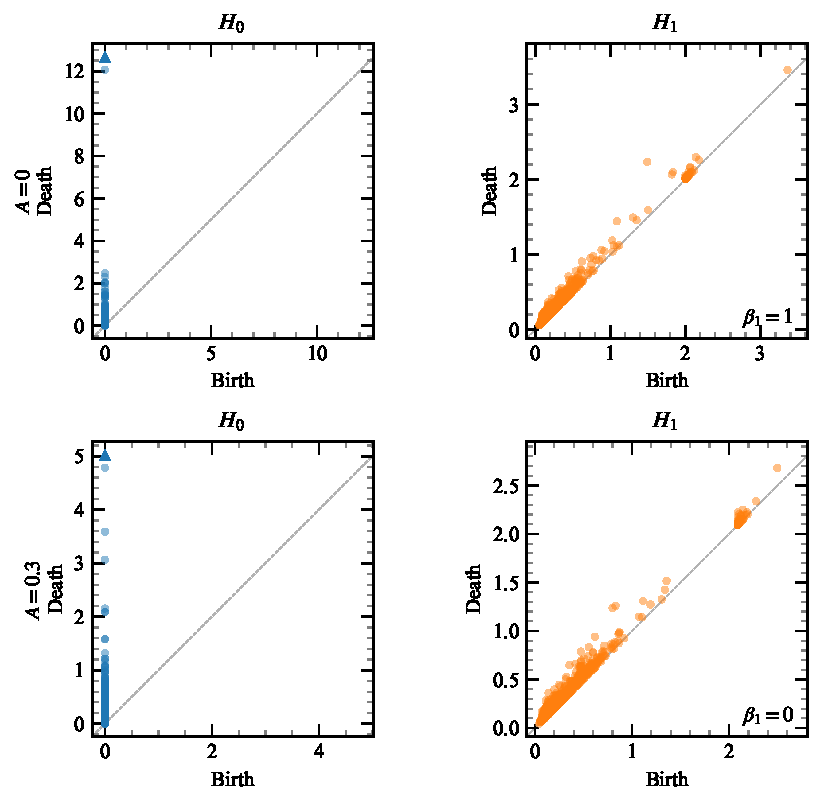
\includegraphics[width=\textwidth]{02.pdf}
\caption{Persistence diagrams for smooth ($A = 0$, top row) and transitional
($A = 0.3$, bottom row) disks.  Left: $H_0$ (connected components); right:
$H_1$ (loops).  Each dot represents a topological feature; its distance from
the diagonal is its persistence (lifetime).  Triangles mark features that
persist to $\infty$ (the single connected component in $H_0$).  The smooth
disk shows one persistent $H_1$ feature ($\beta_1 = 1$), while the
transitional disk shows none ($\beta_1 = 0$).}
\label{fig:persistence}
\end{figure*}

\begin{deluxetable}{ccccc}
\tablecaption{Persistence summary across perturbation amplitudes.
\label{tab:bifurcation}}
\tablehead{
\colhead{$A$} &
\colhead{$H_1$ pers.} &
\colhead{$H_1$ max} &
\colhead{$H_0$ max} &
\colhead{$H_0$ gap}
}
\startdata
0.00 & 1 & 0.743 & 12.067 & 9.595 \\
0.05 & 1 & 0.504 &  8.227 & 5.434 \\
0.10 & 0 & 0.293 &  4.496 & 2.156 \\
0.15 & 0 & 0.394 &  4.398 & 2.328 \\
0.20 & 2 & 0.566 &  4.480 & 2.419 \\
0.25 & 1 & 0.584 &  2.495 & 0.249 \\
0.30 & 0 & 0.437 &  4.782 & 1.192 \\
\enddata
\tablecomments{$H_1$ pers.: number of $H_1$ features with lifetime $> 0.5$.
$H_1$ max: maximum $H_1$ lifetime.
$H_0$ max: maximum $H_0$ lifetime (in standard deviations after log-transform
and scaling).
$H_0$ gap: difference between 1st and 2nd $H_0$ lifetimes.
$N = 4000$ systems per value of $A$.  All features computed after log1p
transform on $M_\text{terr,tot}$, $\bar{M}_\text{terr}$, and $\eta$.}
\end{deluxetable}

\begin{figure}
\centering
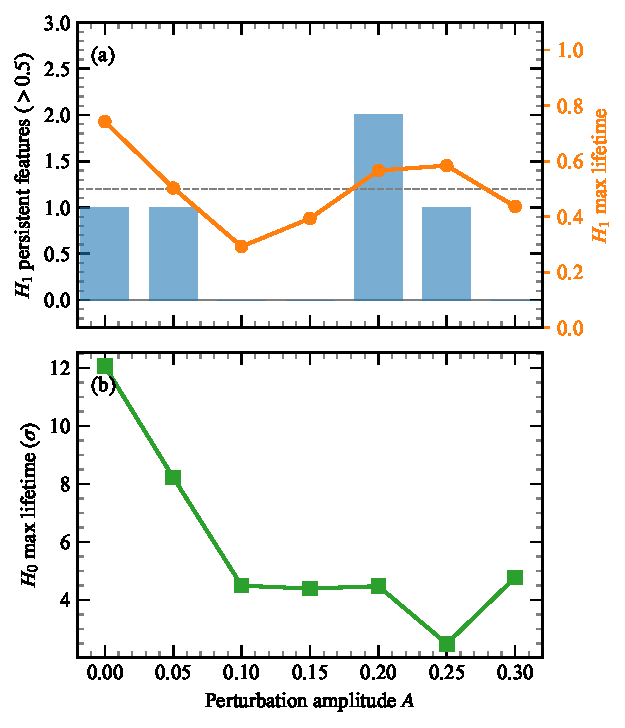
\includegraphics[width=\columnwidth]{03.pdf}
\caption{Bifurcation diagram.  (a)~Number of persistent $H_1$ features
(bars, left axis) and maximum $H_1$ lifetime (orange line, right axis) as a
function of perturbation amplitude $A$.  The dashed line marks the persistence
threshold (0.5).  (b)~Maximum $H_0$ lifetime, showing softening of the
dominant cluster separation.  $N = 4000$ systems per value of $A$.}
\label{fig:bifurcation}
\end{figure}

\subsubsection{$H_1$: degeneracy resolution}
\label{sec:h1}

The smooth disk ($A = 0$) exhibits one robust persistent $H_1$ loop (lifetime
0.74), indicating an irreducible degeneracy in the inverse problem:
topologically distinct families of disk initial conditions produce
architecturally indistinguishable planetary systems.  As $A$ increases, this
degeneracy is resolved:
\begin{equation}
\beta_1: \quad 1 \to 1 \to 0 \to 0 \to 2 \to 1 \to 0.
\end{equation}
Three \textbf{degeneracy-free windows} appear at $A = 0.1$, $A = 0.15$, and
$A = 0.3$, where $\beta_1 = 0$ at the 0.5 threshold.  In these windows, the
inverse problem is topologically well-posed: every planetary architecture maps
to a connected region of disk initial conditions.

The transient reappearance of $H_1$ features at $A = 0.20$--$0.25$ reflects
the interplay between the cosine perturbation structure
(Equation~\ref{eq:perturbation}) and the characteristic scales of planet
formation (snow line, isolation mass).  As $A$ increases, the radial positions
of over-dense and under-dense regions shift relative to these critical radii,
creating and then resolving different formation pathway degeneracies.

\subsubsection{$H_0$: cluster softening}
\label{sec:h0}

The dominant $H_0$ lifetime generally decreases from 12.1 ($A = 0$) to
$\sim$4.5 ($A \geq 0.1$).  The large value at $A = 0$ is driven by a small
number of systems with extreme $N_\text{giant}$ (up to 7 giant planets); the
gap between the first and second $H_0$ lifetimes drops from 9.6 to $\sim$1--2
across the sweep.

Despite the sensitivity of the dominant $H_0$ feature to rare extreme systems,
the overall trend is clear: the density perturbation \textbf{softens} the
cluster structure, reducing the separation between the most distinct
populations as intermediate formation pathways emerge from the density
modulation.

\subsubsection{Classification invariance}
\label{sec:invariance}

The giant planet fraction remains stable at $31.1$--$31.7\%$ across all
values of $A$.  The topological changes are \textbf{not driven by shifts in
population fractions} but by reorganization of the internal geometry of the
outcome space.  This is precisely the structure that KDE-on-marginals cannot
detect: the marginal distributions are nearly identical, but the topology
differs.

% ===========================================================================
% DISCUSSION
% ===========================================================================
\section{Discussion}
\label{sec:discussion}

The central result of this work is that the perturbation amplitude $A$ acts as
a bifurcation parameter for the topology of the planetary architecture space.
This has several implications:

\textbf{For disk archeology:} The existence of an $H_1$ loop at $A = 0$ means
that certain planetary architectures have genuinely multiple formation
histories --- the inverse problem is ill-posed in those regions regardless of
observational precision.  The resolution of this degeneracy at $A \geq 0.1$
suggests that disk substructure (dust traps, density perturbations) provides
sufficient additional information to break the degeneracy.  This has practical
implications for exoplanet surveys: systems that formed in transitional disks
may be more amenable to archeological reconstruction than those from smooth
disks.

\textbf{For population synthesis:} The topological changes occur while the
classification fractions remain invariant.  This demonstrates that persistent
homology captures structure in the forward map that is invisible to
population-level statistics.  Future population synthesis studies should
consider topological invariants alongside traditional metrics.

\textbf{Preprocessing is critical:} The consolidated architecture features
($M_\text{terr,tot}$, $\bar{M}_\text{terr}$, $\eta$) are approximately
log-normally distributed, spanning orders of magnitude.  Without
log-transformation, linear standardization produces artificial outlier
structure that inflates the apparent topological complexity (4 spurious $H_1$
loops vs.\ 1 robust loop).  This underscores that TDA results on population
synthesis data are sensitive to preprocessing choices, and that the underlying
distribution of summary statistics must be accounted for before computing
persistence.

\textbf{Limitations:} Our model uses a parameterized Kelvin--Helmholtz
timescale rather than solving the full envelope structure equations, and
employs the Tanaka Type~I migration formula rather than the Paardekooper
torques with corotation terms.  These simplifications affect the absolute
classification fractions but are unlikely to change the qualitative topology,
since the formation channels (giant, terrestrial, failed) are robustly
produced.  The solid disk is static (no planetesimal drift), and the gas disk
evolves via simple exponential decay rather than viscous diffusion.  The
dominant $H_0$ feature is sensitive to rare systems with extreme $N_\text{giant}$,
and future work should explore alternative distance metrics or feature
representations that are more robust to discrete-valued dimensions.

% ===========================================================================
% SUMMARY
% ===========================================================================
\section{Summary}
\label{sec:summary}

We have applied persistent homology to the output of semi-analytic population
synthesis simulations to characterize the topological structure of the
protoplanetary disk inverse problem.  Our main findings are:

\begin{enumerate}
\item Smooth disks ($A = 0$) exhibit \textbf{one robust persistent $H_1$
loop} (lifetime 0.74 standard deviations), indicating an irreducible
degeneracy where topologically distinct disk configurations produce
indistinguishable planetary architectures.

\item The density perturbation amplitude $A$ acts as a \textbf{bifurcation
parameter} that resolves this degeneracy, with $\beta_1 = 0$ at $A = 0.1$,
$0.15$, and $0.3$.

\item The dominant $H_0$ cluster separation \textbf{softens} with $A$,
indicating that dust traps create intermediate formation pathways between
the most distinct populations.

\item These topological changes are \textbf{independent of the population
fractions}, which remain invariant at $\sim$31\% giant planet systems across
all values of $A$.

\item \textbf{Preprocessing matters}: log-transformation of the mass-related
features is essential for reliable persistence computation on population
synthesis data.  Without it, the heavy-tailed distributions produce spurious
topological features.
\end{enumerate}

The code, infrastructure, and documentation for this project are publicly
available at \url{https://github.com/caverac/topological-archeology}.

% ===========================================================================
\begin{acknowledgments}
The simulations were performed on AWS Lambda.  Persistent homology was computed
using Ripser \citep{Bauer2021}.  This work made use of NumPy and SciPy.
\end{acknowledgments}

\bibliography{ms}

\end{document}
